\section{Hyperfine Dips}
\label{sec:hyperfine}
Firstly we want to show all absorption dips separately starting with peak 1 and ending with peak 4.
\begin{center}
    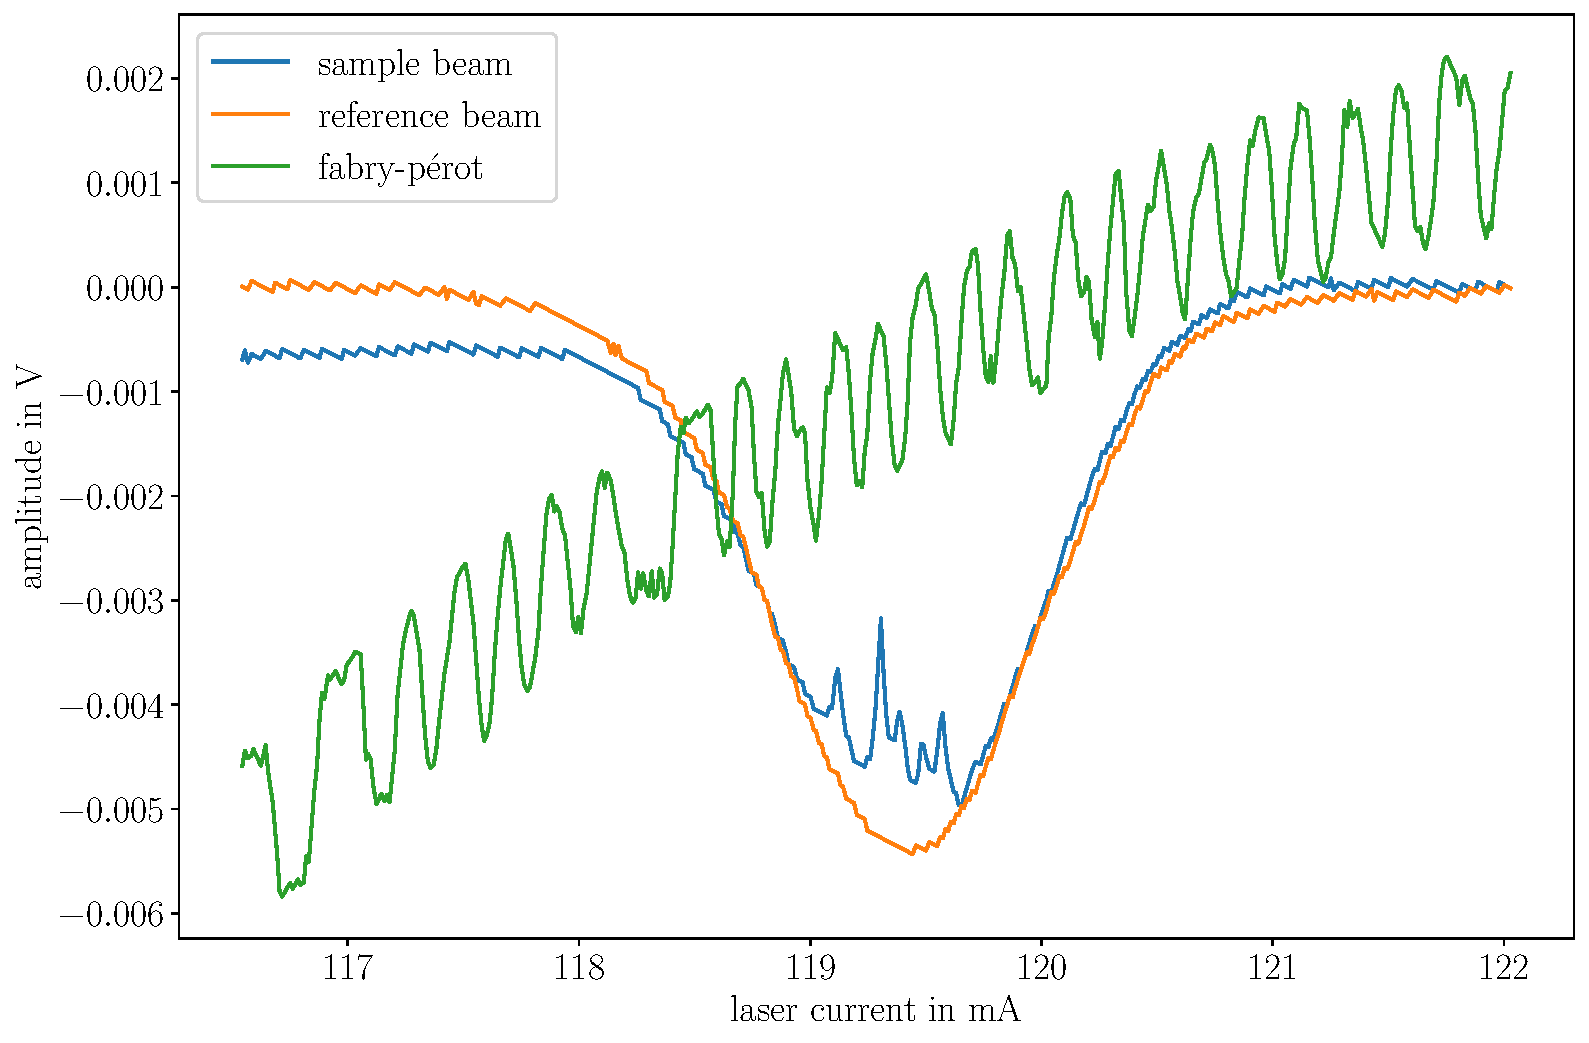
\includegraphics[scale=0.45]{Aufg-4/hyperfine1.pdf}
    \captionof{figure}{absorption spectrum of peak number 1}
    \label{image:peak1}
\end{center}
\begin{center}
    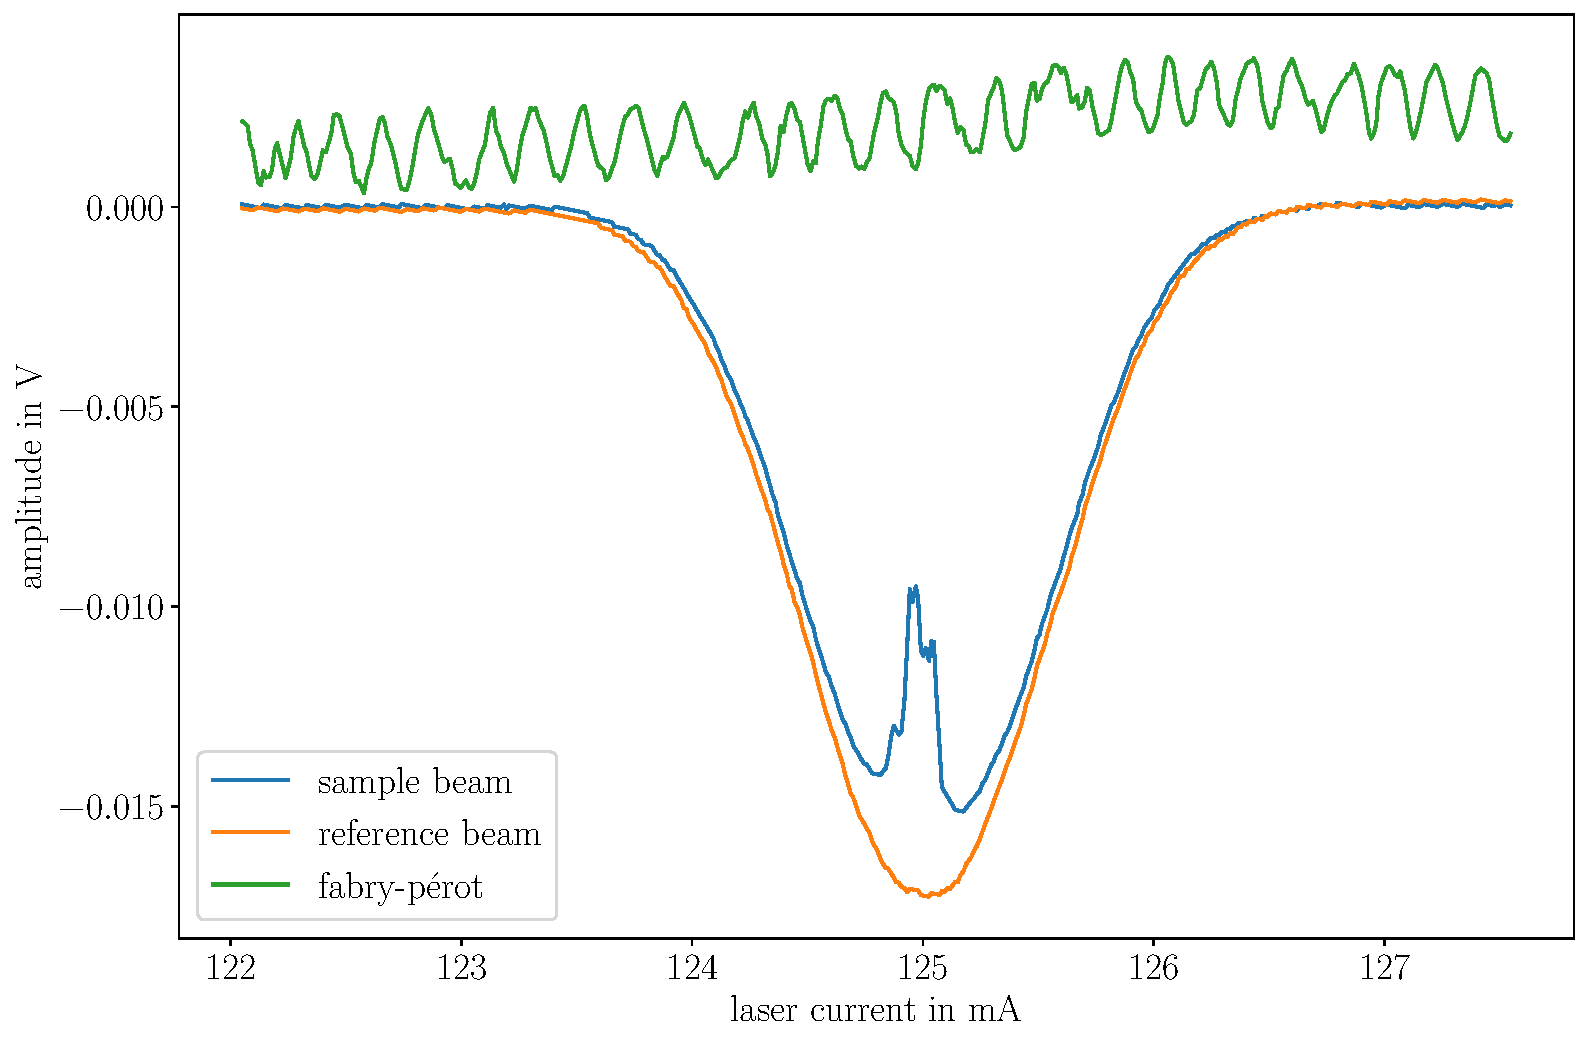
\includegraphics[scale=0.45]{Aufg-4/hyperfine2.pdf}
    \captionof{figure}{absorption spectrum of peak number 2}
    \label{image:peak2}
\end{center}
\begin{center}
    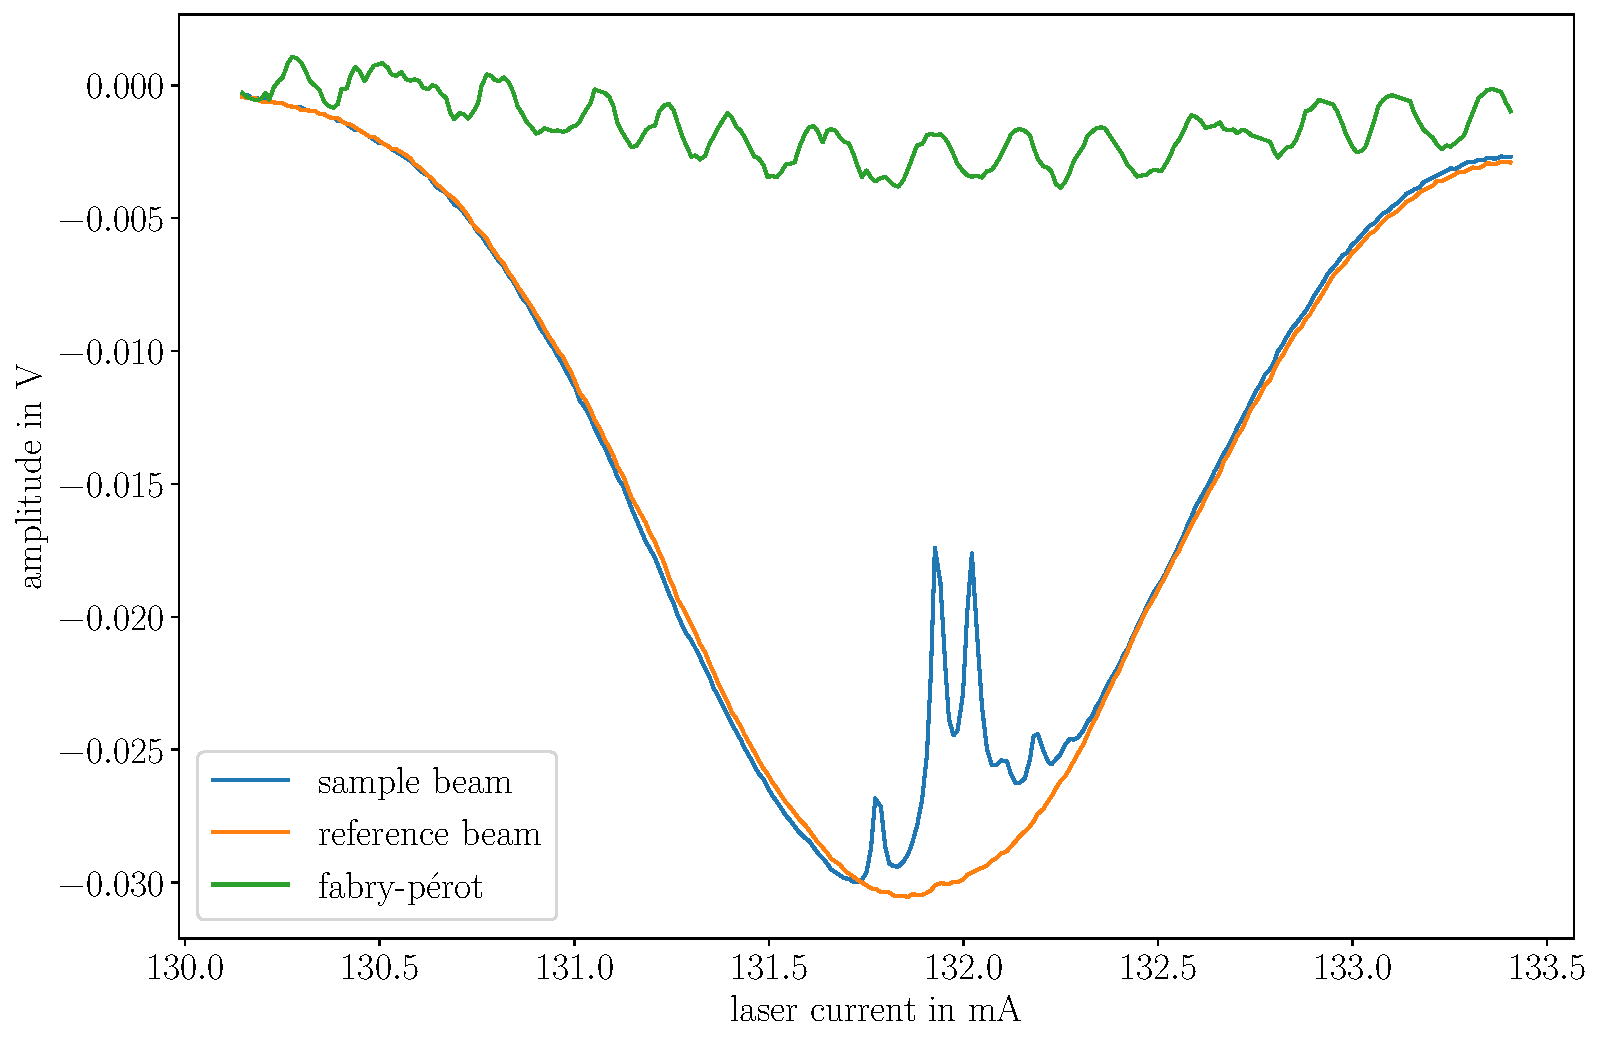
\includegraphics[scale=0.45]{Aufg-4/hyperfine3.pdf}
    \captionof{figure}{absorption spectrum of peak number 3}
    \label{image:peak3}
\end{center}
\begin{center}
    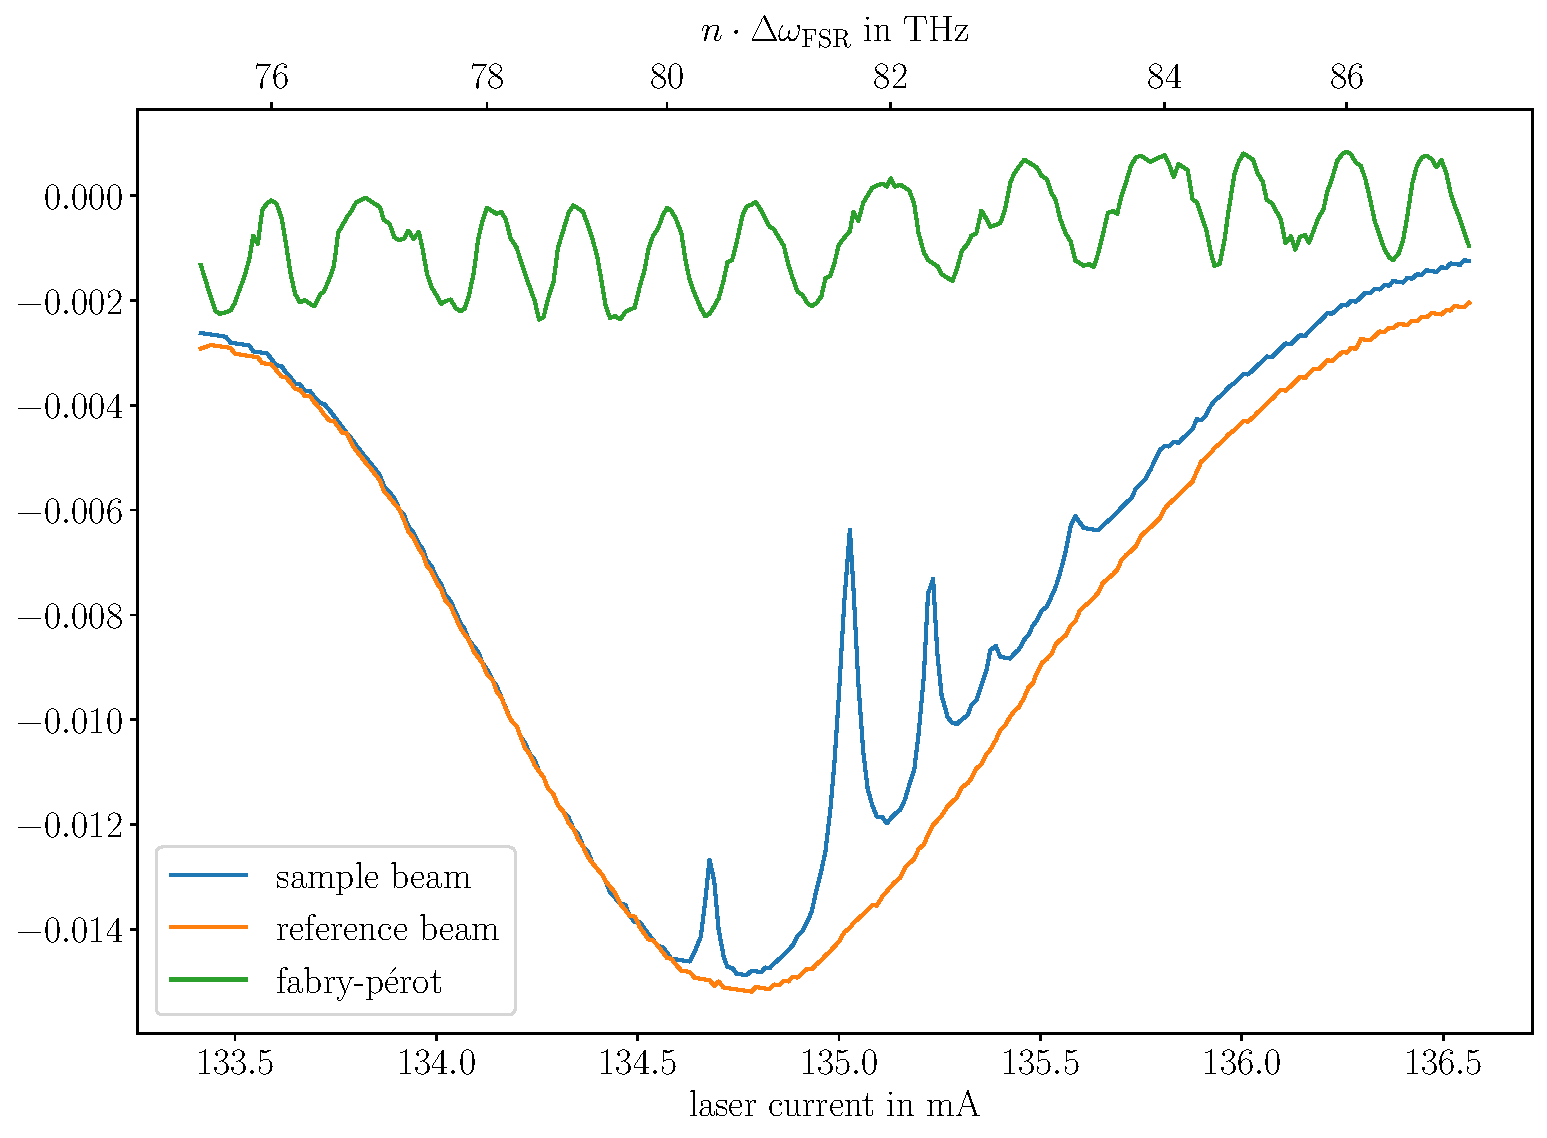
\includegraphics[scale=0.45]{Aufg-4/hyperfine4.pdf}
    \captionof{figure}{absorption spectrum of peak number 4}
    \label{image:peak4}
\end{center}
\newpage
It was chosen to use the peak number 3 because there are the hyperfine dips clearly visible. Its the isotope $^{85}Rb$. For the upcuming calculation we will use the measured data of peak 3 only because of that we have had an offset in our data from $z_{off}=\SI{0.072}{\volt}$ and have to transform the laser current again like in chapter \ref{sec:freeing} into wavelength and frequency.
The fit of the Lorentz curve (lorentzian) was achieved with the function:
\begin{gather}
    y = \frac{a c^2}{(x-b)^2+c^2} - d
\end{gather}
By observing the formula of the fit it gets clear that $a$ is nothing else as the laser current value and $b$ the amplitude of each hyperfine dip peak. From that conclusion we get for the hyperfine peaks numbered from left to right:
\begin{center}
    \begin{tabular}{c | c c c c c c}
        \makecell{hyperfine\\peak} &\makecell{$a$/mA} & $a$/nm &  $a$/THz &  $b$/V & $c$/mA & $d$/V \\
        \hline
        1   &   131.8489  &  780.236290  &  384.232907   &  -0.0269 & -0.0266 & -0.032\\
        2   &   132.0006  &  780.236438  &  384.232834   &  -0.0169 & -0.0285 & -0.032\\
        3   &   132.0778  &  780.236513  &  384.232797   &  -0.0177 & -0.0325 & -0.032\\
        4   &   132.1607  &  780.236594  &  384.232757   &  -0.0254 & -0.0680 & -0.032\\
        5   &   132.2349  &  780.236667  &  384.232722   &  -0.0243 & -0.0613 & -0.032\\
        \end{tabular}
        \captionof{table}{fitting data for each hyperfine dip}
        \label{tab:lorFit}
\end{center}
Furthermore the lorentzian fit for each dip can be seen in fig. \ref{image:lorFit}.\\
It is clear that there are more dips than possible hyperfine transition. In case of $^{85}Rb$ each dip represents a transition from energy levels $F=3$ of the state $5^2S_{1/2}$ to a different energy level of the $5^2P_{3/2}$ state with quantum number $F'$, in short: $F=3\rightarrow F'$. With the selection rule of the hyperfine transition ($\Delta F = 0,\pm1$) we obtain that there should be only three dips visible ($F'=2,3,4$) the remaining dips come from cross over resonances.
For Comparison with the literature \citep{RDL85} we calculate the distance between the dips using table \ref{tab:lorFit} and obtain:
\begin{center}
    \begin{tabular}{c | c c | c c}
        \makecell{dip area} & \makecell{distance\\measured/MHz} & \makecell{distance\\literature/MHz} & \makecell{transition\\ $F'_1\leftrightarrow F'_2$} \\
        \hline
        $1\rightarrow 2$ & 73.00 & 63.38 & $2\leftrightarrow 3$ \\
        $2\rightarrow 5$ & 114.00 & 120.99 & $3\leftrightarrow 4$\\
    \end{tabular}
    \captionof{table}{distance between the selected dips}
    \label{tab:disDip}
\end{center}
The Comparison with the literature shows us that indeed the peek 3 should be $^{85}Rb$ as we assumed in chapter \ref{sec:freeing} and \ref{sec:ratio}. The difference between literature and measurement could have the same cause as the difference in chapter \ref{sec:freeing}.
\newpage
\begin{center}
    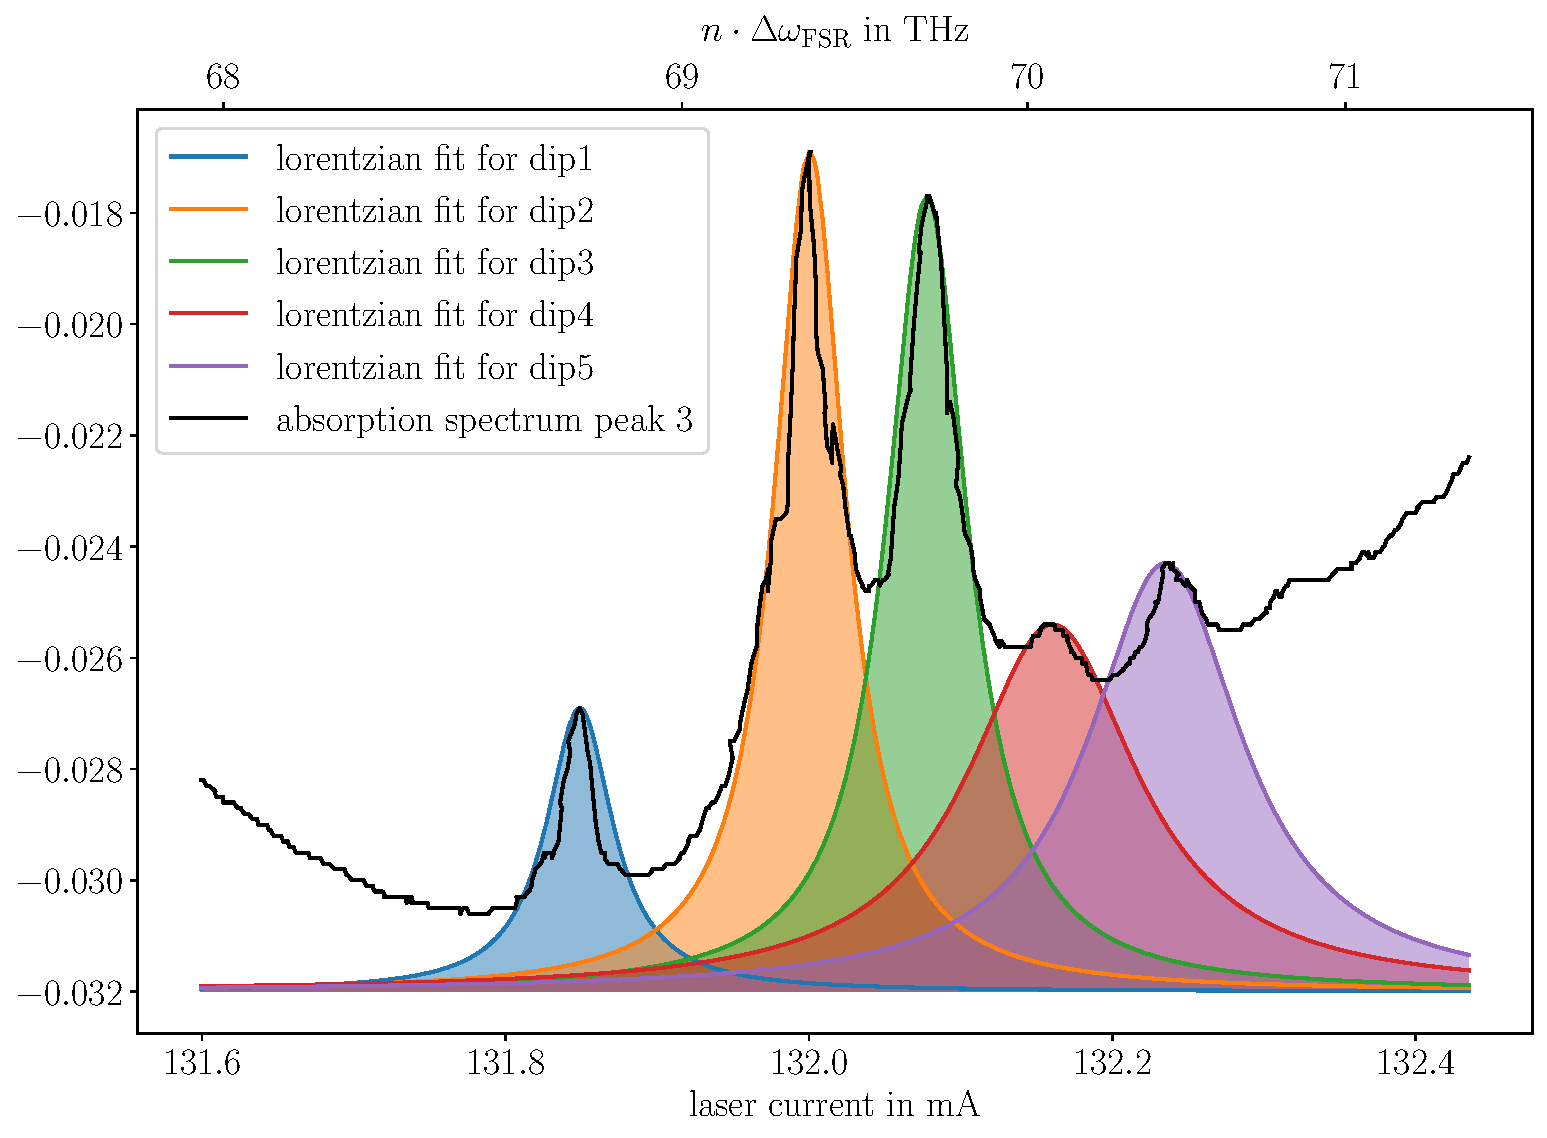
\includegraphics[scale=0.72, angle = 90]{Aufg-4/hyperfinePeak3.pdf}
    \captionof{figure}{lorentzian fit for each dip of peak 3}
    \label{image:lorFit}
\end{center}

%$1\rightarrow 2$ & 73.0 & & \\
%        $2\rightarrow 3$ & 37.0 & & \\
%        $3\rightarrow 4$ & 40.0 & & \\
%        $4\rightarrow 5$ & 37.0 & & \\